\numberwithin{equation}{section}
\numberwithin{table}{section}
\newtheorem{example}{Example}
\section{Preliminaries}
\label{sec:preliminaries}
\subsection{Conjunctive Normal Form}
A formula is said to be in Conjunctive Normal Form (CNF) if and only if it is a conjunction of clauses and a clause is a disjunction of literals. A literal could be a positive or negative instance of Boolean variable. A CNF formula $\varphi$ is defined as follows:
$$\varphi = \bigwedge\limits_{i=1\ldots n} C_{i}$$
$$ C_{i} = \bigvee\limits_{i=1\ldots k_{i}} a_{ij}$$
here, $C_{i}$ is the $i^{\text th}$ clause and $n$ is the number of total clauses in $\varphi$, $a_{ij}$ is a literal and $m$ is the total number of literals in $C_{i}$.\newline
\begin{example}
	Assume the following CNF formula,
	$$\varphi=\underbrace{(x)}\limits_{C_{1}}\wedge\underbrace{(\neg x)}\limits_{C_2}\wedge\underbrace{(\neg x\vee y)}\limits_{C_{3}}\wedge\underbrace{(\neg x \vee \neg y)}\limits_{C_{4}}$$
	where, $x, \neg x, y$ and $\neg y$ are the literals.
\end{example}
The aforementioned CNF formula will ne used as an example throughout this paper which is unsatisfiable.
\subsection{Satisfiability Checking}
Satisfiability checking determines whether the existentially quantified first-order-logic formulas are satisfiable by generating solutions automatically. The formulas are Boolean combinations of theory constraints and the form of theory constraints varies depending on with which theory we want to represent first-order-logic. Some example theory constraints from different theories are given in \cite{erika}. There are two types of solvers for satisfiability checking: $1)$ Boolean satisfiability (SAT) solver and $2)$ SAT-modulo-theories (SMT) solver.\newline
A SAT solver solves the Boolean satisfiability problem (the problem of determining if there exists any satisfying soultion for a given Boolean formula) by implementing decision procedure. The Davis–Putnam–Logemann–Loveland (DPLL) algorithm is the basis for most modern SAT solvers. The input formula of it is expected to be in CNF.\newline
Example: Let us consider a CNF, $(x) \wedge (\neg x\vee\neg y) \wedge (z)$. Boolean constraint propagation (BCP) (determines the assignment of next variable implied by the last decision) starts with $x$ as it is a single literal and $x$ is set to $true$. Then, BCP indicates that  $y$ of the second clause must be $false$ to satisfy the CNF. There is still a unassigned variables. A new decision will be made and $z$ is set to $true$. As all variables are assigned and there is no conflict, the satisfying soluiton is $x=1, y=0$ and $z=1$.\newline
A SMT solver can be applied on quantifier-free first-order-logic formulas with an underlying theory to check the satisfiability. There are two type of SMT solvers, Eager SMT solver and Lazy SMT solver. To know about SMT solver in details you can read \cite{kremer}.
\subsection{Clause-Selector Variables}
Authors of the paper \cite{karem} has used clause-selector variable by augmenting a CNF formula. Clause-selector variable is a variable, $w_{i}$ which is negated to augment each clause of $C_{i}$ of a CNF such that $C^{\prime}_{i}=(\neg w_{i})\vee C_{i}$ in a new formula $\varphi^{\prime}$. Notice that each $C^{\prime}_{i}$ is an implication, $C^{\prime}_{i}=(\neg w_{i}\rightarrow C_{i})$. It means if $w_{i}$ is set to $true$, the original clause $C_{i}$ is being enabled. Conversely, assigning $w_{i}$ $false$ means $C_{i}$ is being disabled or removed from the set of clauses, because $C^{\prime}_{i}$ is satisfied by the assignment of $w_{i}$. So, adding clause-selector variables provides the SAT solver the ability to enable and disable clauses as a part of its normal search.\newline
For our example formula $\varphi=(x)\wedge(\neg x)\wedge(\neg x\vee y)\wedge(\neg x \vee \neg y)$, after adding clause-selector variables we get the following augmented formula $\varphi^{\prime}$, 
$$\varphi^{\prime}=(\neg w_{1}\vee x)\wedge(\neg w_{2}\vee \neg x)\wedge(\neg w_{3}\vee \neg x\vee y)\wedge(\neg w_{4}\vee \neg x \vee \neg y)$$
\subsection{Minimal Unsatisfiable Subset and Minimal Correction Subset}
An Unsatisfiable Subset (US) ia a subset of the clauses of an unsatisfiable CNF formula $\varphi$ where the conjunction of clauses is unsatisfiable. US is said to be Minimal Unsatisfiable Subset (MUS) if and only if removing any clause from UC makes it satisfiable. A Minimal Correction Subset (MCS) is a subset of the clauses of $\varphi$ whose removal from $\varphi$ make it satisfiable and which is minimal. A formula can have multiple MUSes and MCSes. For any formula $\varphi$, MUSes and MCSes of $\varphi$ can be represented as MUSes($\varphi$) and MCSes($\varphi$), respectively. The formal definitions of the set of MUSes and MCSes of $\varphi$ are given in the following:
\begin{definition}[MUS]
	\label{def:mus}
A subset $U$ be a MUS which is a subset of $\varphi$ if $U$ is unsatisfiable and for each clause $C_{i}$ containing in $U$, the removal of $C_{i}$ from $U$ is satisfiable.
$$MUSes(\varphi)
\quad = \quad 
\left\{
\begin{array}{ll}
{\displaystyle U \subseteq \varphi} 
& 
\text{, U is unsatisfiable }
\\[0.6cm] % adjust the line spacing
{\displaystyle\forall C_{i} \varepsilon U} & \text{, U $\backslash \{C_{i}\}$ is satisfiable}
\end{array}
\right.$$
\end{definition}
\begin{definition}[MCS]
	\label{def:mcs}
A subset $M$ be a MCS which is a subset of $\varphi$ if the removal of $M$ from $\varphi$ is satisfiable and for each clause $C_{i}$ containing in $M$ the removal of $M$ from $\varphi$ is unsatisfiable where $M$ does not have $C_{i}$.
$$MUSes(\varphi)
\quad = \quad 
\left\{
\begin{array}{ll}
{\displaystyle M \subseteq \varphi} 
& 
\text{, $\varphi\backslash M$ is satisfiable}
\\[0.6cm] % adjust the line spacing
{\displaystyle\forall C_{i} \varepsilon M} & \text{, $C\backslash(M\backslash\{C_{i}\})$ is unsatisfiable}
\end{array}
\right.$$
\end{definition}
For our example formula $\varphi=(x)\wedge(\neg x)\wedge(\neg x\vee y)\wedge(\neg x \vee \neg y)$, the MUSes and MCSes are shown in the Table $2.1$.
\begin{table}[]
	\centering
	\caption{All MUSes and MCSes}
	\label{my-label}
	\begin{tabular}{|l|l|}
		\hline
		$MUSes(\varphi)$ & $\{C_{1},C_{2}\},\{C_{1},C_{3},C_{4}\}$ \\ \hline
		$MCSes(\varphi)$ & $\{C_{1}\},\{C_{2},C_{3},C_{4}\},\{C_{2},C_{4}\}$ \\ \hline
	\end{tabular}
\end{table}
\subsection{Hitting Sets}
Assume, $\Omega$ is a collection of sets of a finite set $D$. A hitting set of $\Omega$ is a subset of $D$ such that it contains at least one element from each subset in $\Omega$. Formally, the definition is given below:\newline
Definition: A hitting set $H$ of $\Omega$ is $H\subseteq D$ such that $\forall S\in \Omega$, $H\cap S\neq 0$ where $S$ represents each subset of $\Omega$.\newline
In the paper \cite{karem}, authors refer to minimal hitting sets which are the hitting sets from which no elements cannot be removed and if at least one element is removed, it will not be a hitting set anymore.\newline
\begin{example}
Let us consider, $\Omega=\{\{a, b\}, \{b, c, d\}\}$. Then, $\{a,b\}, \{b,c,d\}, \{a,c,d\}, \{b\},\cdots$ are the hitting sets where, $\{b\}$ is the only minimal hitting set.	
\end{example}
\subsection{MUS $\backslash$ MCS Duality}
There is a relationship between MUSes and MCSes which is the foundation of paper \cite{karem}. The relationship states that the set of MUSes of formula $\varphi$ is equal to the set of minimal and irreducible hitting sets of the set of MCSes and vice-versa. This is the duality of MUS and MCS. Formally, it can said that:
\begin{enumerate}
	\item A subset $U$ of $\varphi$ is an MUS if and only if $U$ is an irreducible hitting set of MCSes$(\varphi)$.
	\item A subset $M$ of $\varphi$ is an MUS if and only if $M$ is an irreducible hitting set of MUSes$(\varphi)$.
\end{enumerate}
\begin{figure}[htb] % where to insert the figure: h=here, t=top, b=bottom,
	% the order htb shows which position is preffered
	\begin{center}
		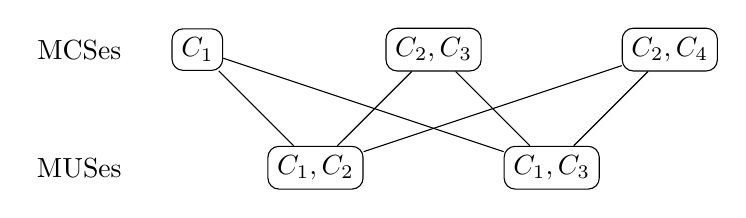
\begin{tikzpicture}[scale=1.5, 
				    state/.style={draw, rounded corners, fill=none,
				    			  text centered, text=black}]
	\node[] (u0) at (1, 2) {MCSes};
	\node[state] (u1) at (2, 2) {$C_{1}$};
	\node[state] (u2) at (4, 2) {$C_{2}, C_{3}$};
	\node[state] (u3) at (6, 2) {$C_{2}, C_{4}$};
	\node[state] (u4) at (3, 1) {$C_{1}, C_{2}$};
	\node[state] (u5) at (5, 1) {$C_{1}, C_{3}$};
	\node[] (u6) at (1, 1) {MUSes};
	
	\path[-] 	(u1)  edge   (u4);
	\path[-] 	(u1)  edge   (u5);
	\path[-] 	(u2)  edge   (u4);
	\path[-] 	(u2)  edge   (u5);
	\path[-] 	(u3)  edge   (u4);
	\path[-] 	(u3)  edge   (u5);

\end{tikzpicture}

	\end{center}
	\caption{Duality of MUSes and MCSes.}
	\label{fig:graph}
\end{figure}
To show duality we use our example formula $\varphi=(x)\wedge(\neg x)\wedge(\neg x\vee y)\wedge(\neg x \vee \neg y)$. First, take the set MCSes of $\varphi$ and it is $\{\{C_{1}\}, \{C_{2}, C_{3}\}, \{C_{2}, C_{4}\}\}$. For this, the set of minimal and irreducible hitting sets is $\{\{C_{1}, C_{2}\}, \{C_{1}, C_{3,} C_{4}\}\}$ which is exactly like the set of MUSes (given in Table $1$). Similarly, we can show that the set of MCSes is the set of irreducible hitting sets of the set of MUSes. So, every MCS has at least one clause from every MUS and vice-versa. The duality is illustrated in Figure(1).
\subsection{AtMost Constraints}
AtMost Constraint is a type of counting clause that can be generated from many types of clauses. If $\{l_{1}, l_{2}, l_{3},\cdots ,l_{\text n}\}$ is a set of $n$ literals and $k$ is a positive integer, an AtMost constraint is defines as,\newline
$$AtMost(\{l_{1},l_{2},\ldots,l_{n}\},k)\equiv \sum\limits^{n}_{i=1} val(l_{i})\leqslant k$$
where, $val(l_{\text i})$ is 1 if $l_{i}$ is assigned $true$ and otherwise 0. $k$ is a bound which tells that maximum how many literals can be assigned $true$.\newline
Authors used an implementation of the AtMost constraints where the variables are watched and propagates the negation of each literal when $k$ of them are assigned $true$. This is implemented with exactly $n$ watched literals and a counter that is incremented or decremented whenever one of them is assigned or unassigned.\newline
Example:Let us consider we have three literals, $l_{1}, l_{2}$,$l_{3}$ and $k=2$. If we call AtMost, we get a clause, $C_{AB}=(l_{1}\vee l_{2}\vee l_{3})$. Here, to make $C_{AB}$ satisfiable exactly two variables can be assigned $true$ as bound is $2$. After that the third variable will be assigned $false$. So, the satisfying soluiton could be $(l_{1}=true, l_{2}=true$ and $l_{3}=false)$ or $(l_{1}=true, l_{3}=true$ and $l_{2}=false)$ or $(l_{2}=true, l_{3}=true$ and $l_{1}=false)$.
